\chapter{Methodology}
\label{ch:methodology}

This chapter describes the methodology used to develop a computer-vision pipeline
for interaction-point perception in hospital environments. The project is conducted
with the objective of building a scalable and deployment-oriented perception system
that can be iteratively improved across different hospital settings and reused
within a robot fleet.

\section{Overview of the proposed perception pipeline}

The proposed methodology focuses on instance-level localization of interaction
elements such as elevator buttons and control panels. Instance segmentation is used
to detect individual button instances at pixel level, allowing precise localization
and separation of closely spaced elements. This capability provides the basis for
subsequent interpretation of button functions and autonomous interaction.

The methodology is designed to support an iterative training and deployment
workflow. An initial base model is deployed on the robot, where it performs
interaction-point perception and collects visual data during operation. Selected
data can be transferred to an offboard system, where annotations may be reviewed,
corrected, or extended before retraining the perception models. The updated models
are then redeployed to the robot and become the new default for continued operation.

This workflow enables gradual adaptation to new hospital environments and allows
knowledge acquired in one deployment to be reused and refined in subsequent
deployments. The target end-to-end training and deployment process toward which this
project is developed is illustrated in Figure~\ref{fig:scalable_workflow}.

The following sections describe each stage of the methodology in detail, beginning
with dataset selection and preparation.
\begin{figure}[htbp]
    \centering
    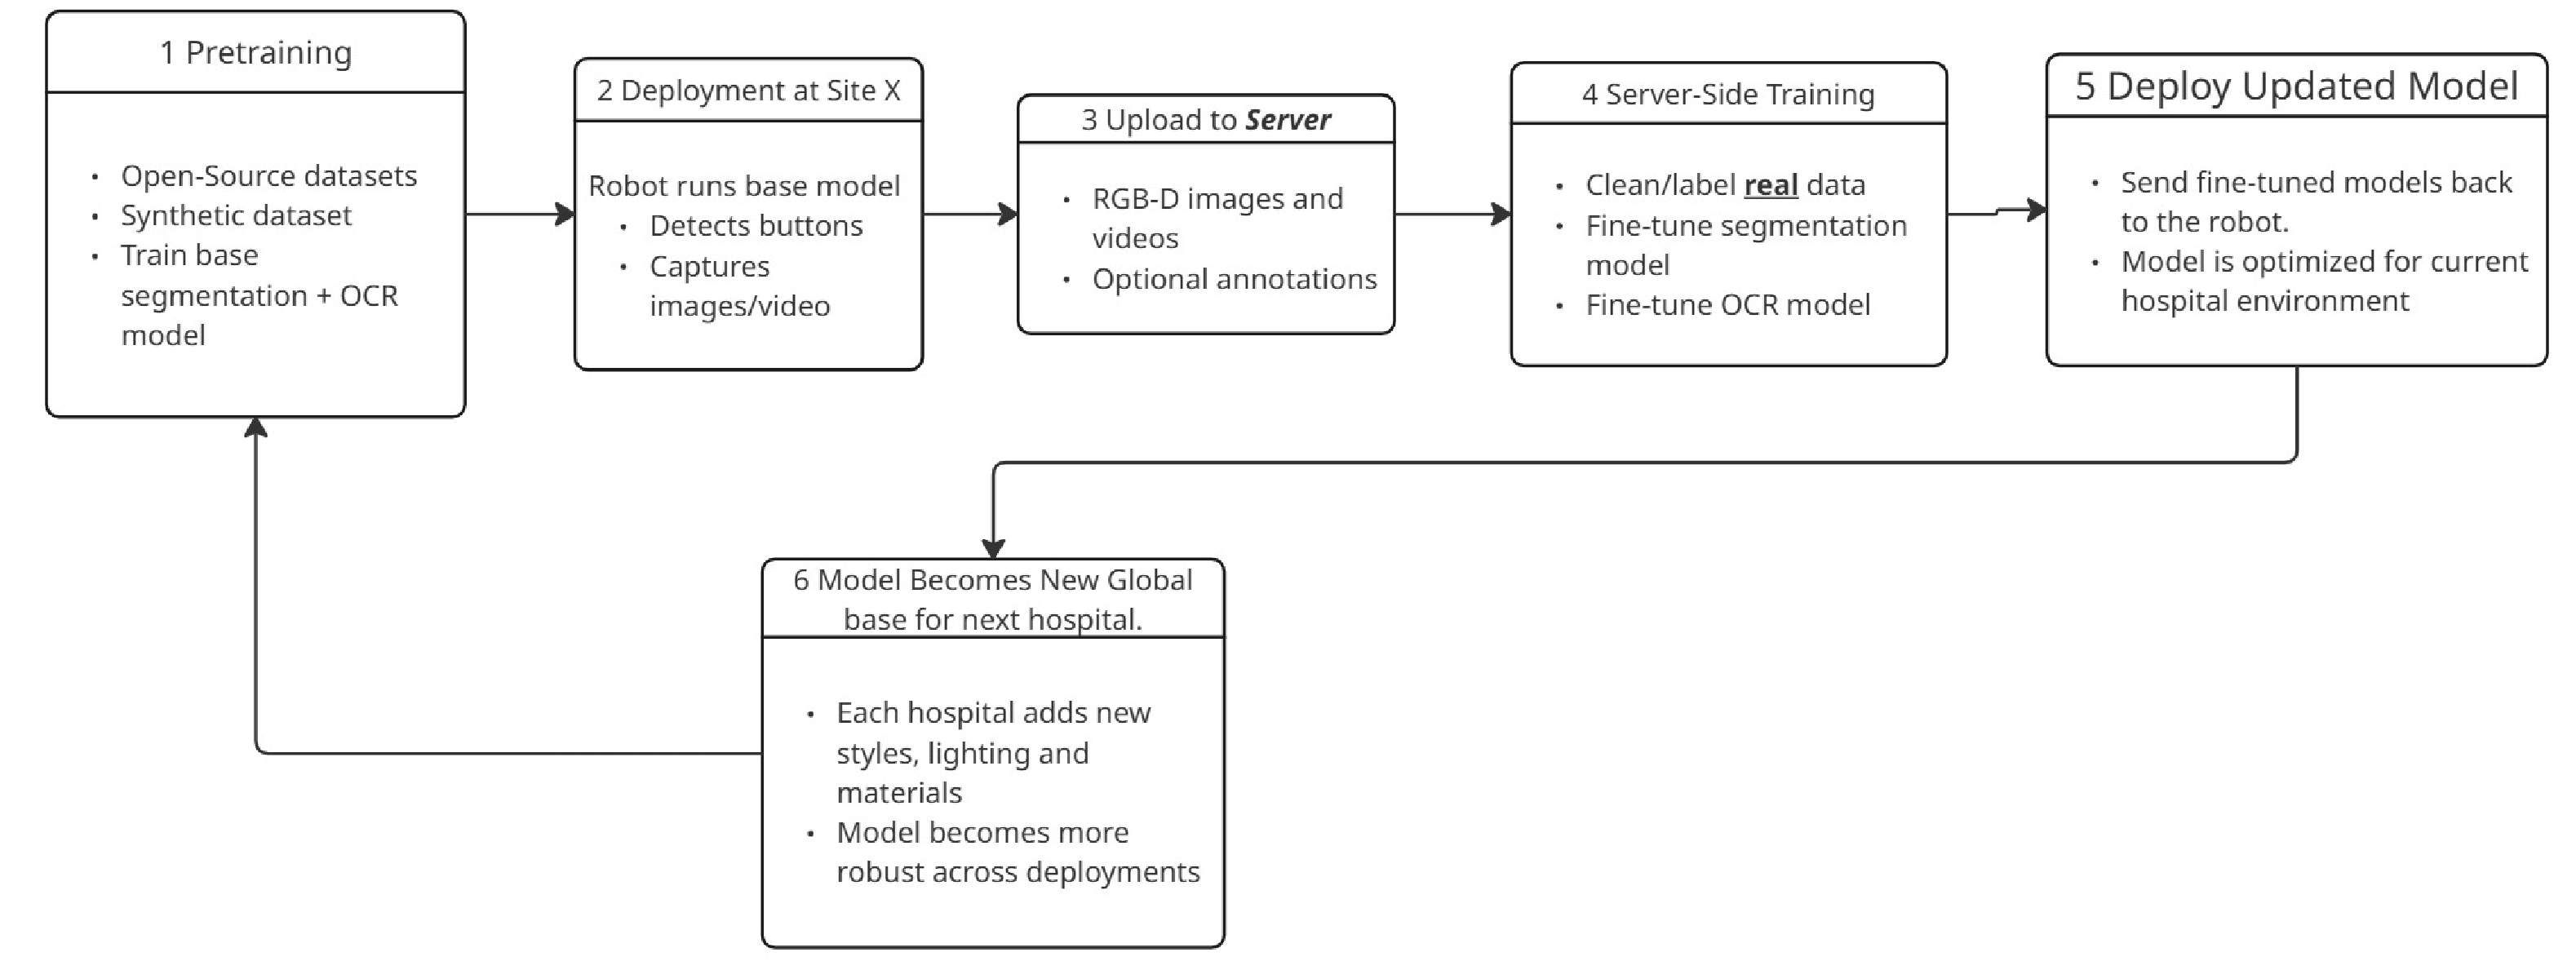
\includegraphics[width=1.1\textwidth]
    {figures/CareBot_workflow.pdf}
    \caption{Target workflow for scalable training and deployment of
    interaction-point perception models across multiple hospital environments.}
    \label{fig:scalable_workflow}
\end{figure}

\section{Dataset selection and preparation}

This project uses a dataset derived from the IRSO2018 collection, which contains
images of elevator panels and buttons captured in realistic indoor environments.
This section corresponds to the initial model-development step in
Figure~\ref{fig:scalable_workflow}, detailing the dataset and its preparation
before the first training cycle.
The origin and relevance of this dataset were discussed in \nameref{ch:literature};
therefore, this section focuses on its structure and preparation for use in this
project.

The dataset consists of a total of 2000 images. Of these, 1400 images are assigned
to the training set (\texttt{train\_set}) and 600 images to the test set
(\texttt{test\_set}). Each subset follows the same directory structure, containing
an \texttt{images} folder with the raw \gls{rgb} images and an \texttt{annotations} folder
with the corresponding annotation files.

In the original dataset, annotations were provided as bounding boxes stored in \gls{xml}
format. For the purposes of this project, the directory structure was preserved,
but the annotation format was replaced with \gls{coco}-style JSON files to support
instance-level segmentation. This ensures compatibility with modern instance
segmentation frameworks while maintaining a clear separation between training and
test data.
\begin{figure}[htbp]
    \centering
    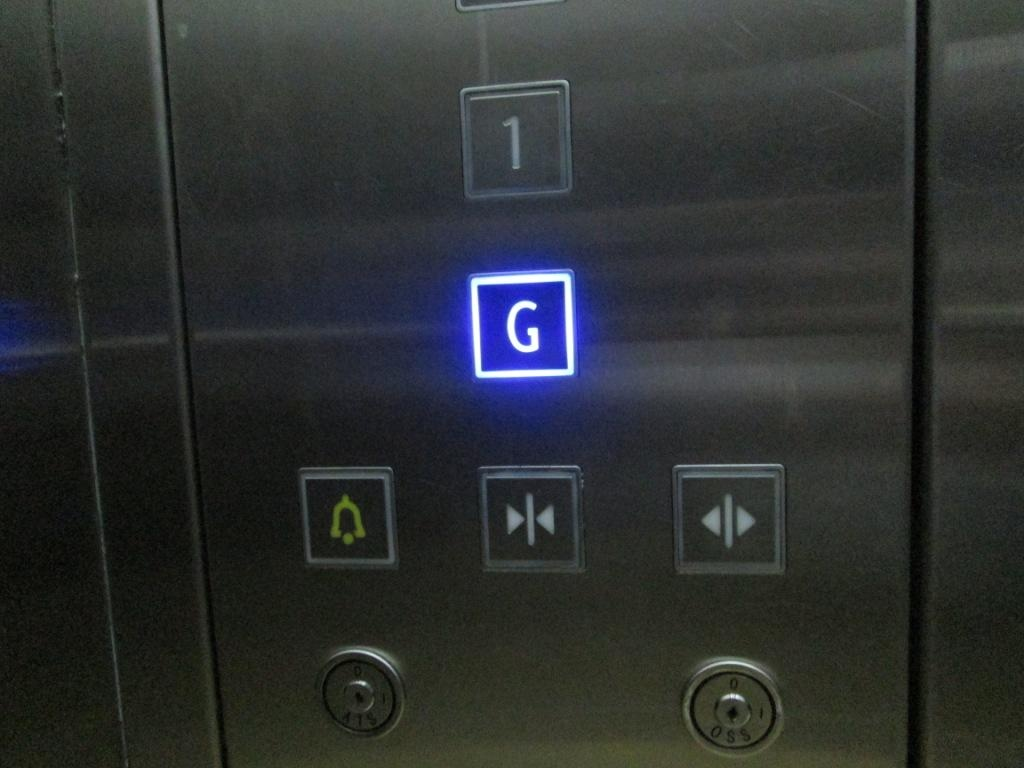
\includegraphics[width=0.4\textwidth]
    {figures/methodology/71.jpg}
    \caption{Example raw image from the dataset.}
    \label{fig:example_raw_image}
\end{figure}

The resulting dataset structure provides a consistent and reusable foundation for
annotation, model training, and evaluation, as described in the following sections.

\section{Annotation strategy and workflow}

Instance-level ground truth was created using a semi-automatic workflow that
combines model-based pre-annotation with manual verification. This strategy was
used to efficiently generate high-quality instance segmentation annotations while
maintaining consistency across the dataset.

Annotations were created in \gls{cvat} \citep{cvat2020}, deployed locally using Docker
\citep{merkel2014docker} within a \gls{wsl}-based Linux environment on a Windows host. Automatic annotation was enabled through \gls{cvat}--Nuclio integration, where the model
was deployed as a Nuclio serverless function \citep{nuclio}. The instance
segmentation model used for automatic annotation was \gls{maskrcnn} \citep{he2017maskrcnn}.

During automatic annotation, \gls{cvat} sends task images to the Nuclio function, where
\gls{maskrcnn} predicts binary masks for each detected button instance. These masks
are converted into polygon shapes within the Nuclio function and returned to \gls{cvat}
as annotation data. The overall workflow used in this project is shown in
Figure~\ref{fig:annotation_workflow}.

\begin{figure}[htbp]
    \centering
    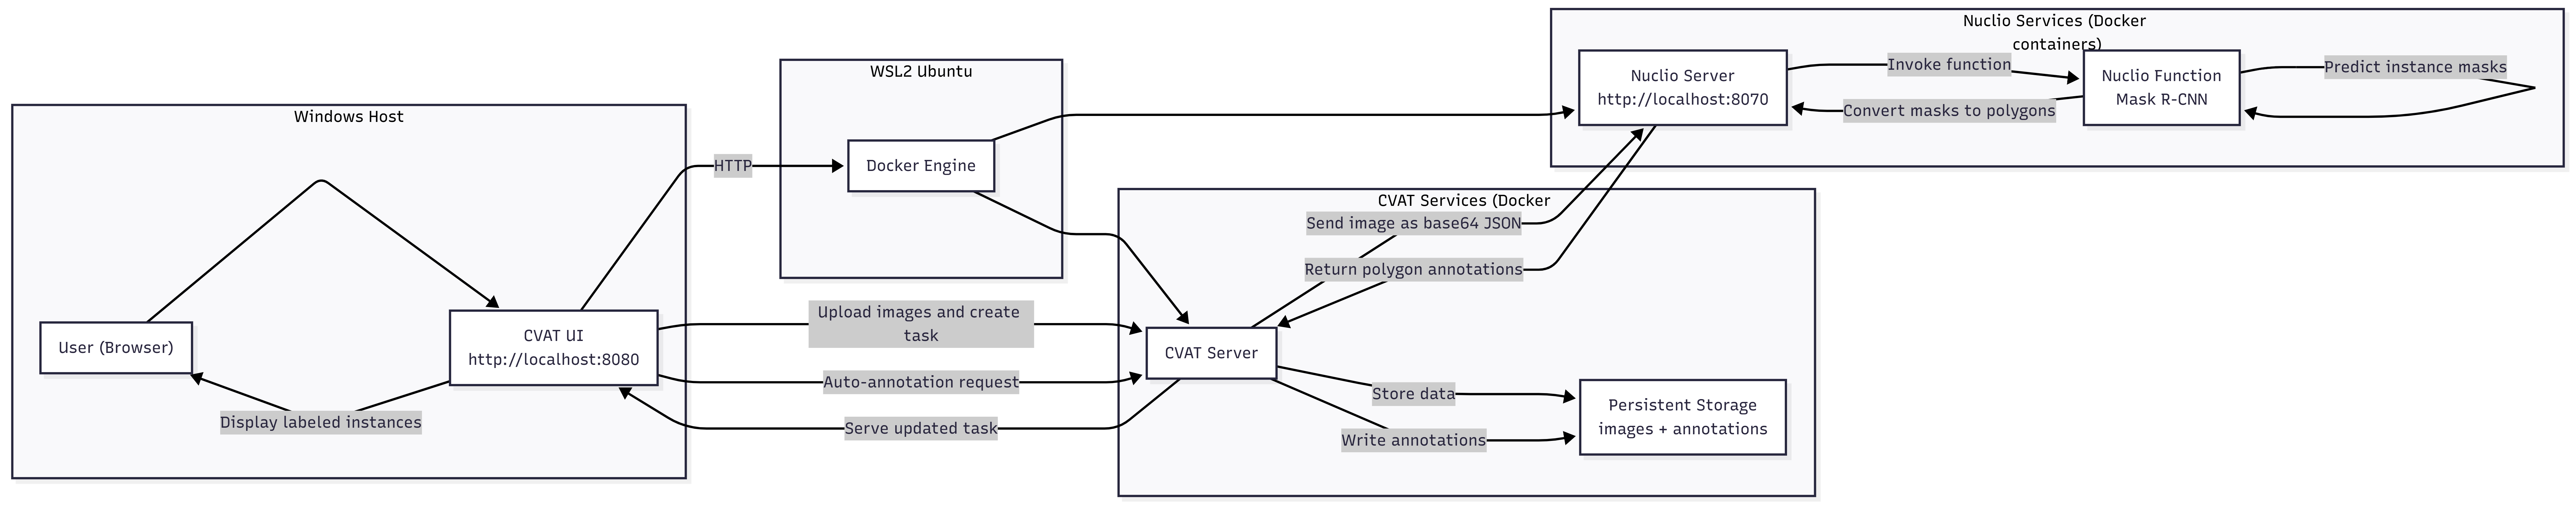
\includegraphics[width=1.3\textwidth]{figures/methodology/Docker_CVAT_Nuclio.png}
    \caption{Semi-automatic annotation workflow on a Windows host using \gls{wsl} and
    Docker. \gls{cvat} sends images to a Nuclio function running \gls{maskrcnn}, which returns
    polygon instance annotations derived from predicted binary masks.}
    \label{fig:annotation_workflow}
\end{figure}

To support iterative improvement, the dataset was annotated in batches of
approximately 150 images. After each batch, the model was retrained using the
newly annotated data and reused for subsequent annotation rounds. Model checkpoints
were created after approximately 100, 450, and 900 annotated images, enabling
progressively improved pre-annotations and reduced manual correction effort.

All automatically generated annotations were also manually reviewed and corrected when needed to
ensure accurate instance boundaries, correct separation of adjacent buttons, and
consistent labeling across both the training and test sets.

\begin{figure}[htbp]
    \centering
    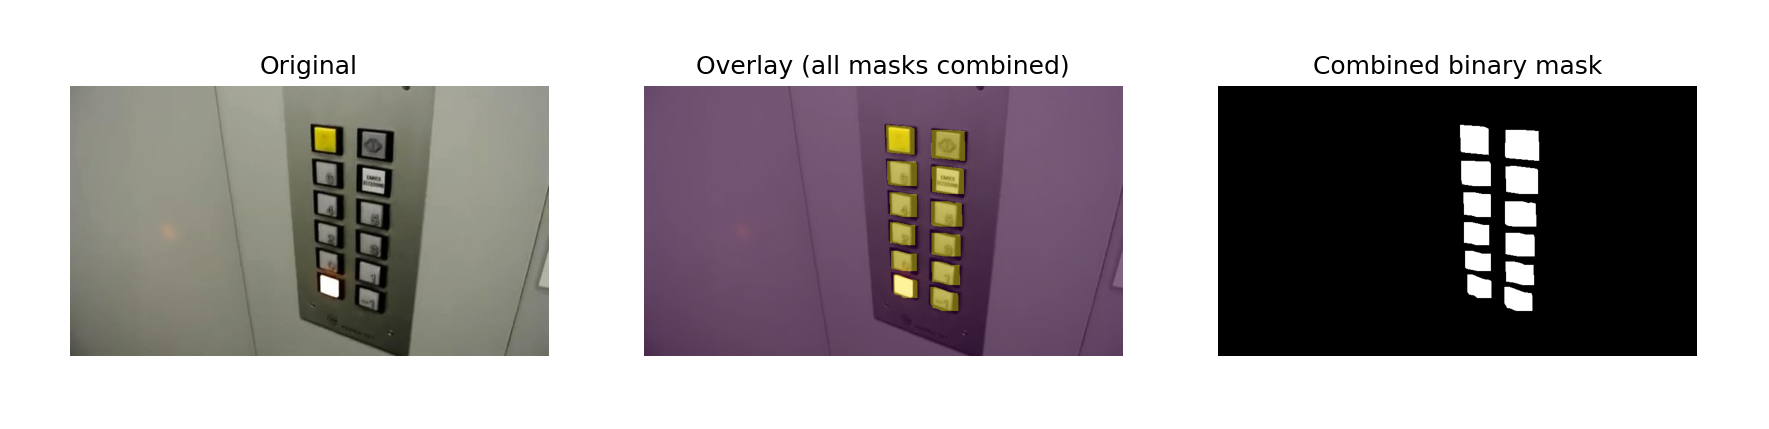
\includegraphics[width=0.95\textwidth]{figures/methodology/instances_Train_1349_1402__971.jpg.png}
    \caption{Example of an annotated image showing instance segmentation masks.}
    \label{fig:example_annotated_image}
\end{figure}

\section{Dataset quality assessment.}
\textbf{Note: This section is not done, and the text within it will most probably be changed drastically. However, I intent to keep structure and general idea the same.
One subsection for model assisted image quality assessment, and one for statistical image quality metrics.}

A systematic dataset quality assessment was performed to verify whether image-level degradation could negatively affect model performance.

\subsection{Statistical quality metrics.}
For every image, the following metrics were computed:
\begin{itemize}
    \item \textbf{Sharpness}, estimated using the variance of the Laplacian:
    \begin{equation}
        \sigma^2_{\text{lap}} = \mathrm{Var}(\nabla^2 I)
    \end{equation}
    where $I$ is the grayscale image.
    \item \textbf{Brightness}, defined as the mean grayscale intensity.
    \item \textbf{Edge density}, defined as the fraction of pixels with gradient magnitude above the 90th percentile.
\end{itemize}

% \paragraph{Results.}
% Figure~\ref{fig:quality_distributions} shows the distributions of sharpness, entropy, and brightness.
% The dataset exhibits predominantly well-exposed images with high information content and moderate sharpness.
% No distinct group of severely degraded images was observed.

% Figure~\ref{fig:quality_vs_performance} shows the relationship between image quality metrics and model performance.
% No strong correlation was found between sharpness or entropy and segmentation quality.
% False positives were primarily associated with low edge density, indicating visually ambiguous but valid scenes rather than image degradation.

% \paragraph{Conclusion.}
% The analysis indicates that dataset quality is high and does not constitute a limiting factor for model performance.
% Quality-based dataset pruning was therefore not applied.

---

\subsection{Model-assisted image assessment.}

In addition to image-level quality analysis, a model-assisted approach was used to identify potentially harmful training samples.

\paragraph{Method.}
A trained instance segmentation model was used to evaluate each training image individually.
For each image, the following metrics were computed:
\begin{itemize}
    \item Mean Intersection over Union:
    \begin{equation}
        \mathrm{IoU} = \frac{|M_{\text{pred}} \cap M_{\text{gt}}|}{|M_{\text{pred}} \cup M_{\text{gt}}|}
    \end{equation}
    \item Mean detection confidence:
    \begin{equation}
        \bar{c} = \frac{1}{N} \sum_{i=1}^{N} p_i
    \end{equation}
    where $p_i$ is the softmax score of the $i$-th predicted instance.
    \item Number of false positives and false negatives.
\end{itemize}

Images were ranked using a composite criterion favoring low \gls{iou}, high false positives, and high confidence incorrect predictions. Based on those criteria, a harm-score is measured,
based on which training set images are filtered and the potentially harmful ones are selected for manual inspection.

\paragraph{Inspection.}
Manual inspection of the lowest-ranked samples revealed two categories:
\begin{itemize}
    \item Hard but valid images (extreme viewpoints, zoom levels, or geometric distortions).
    \item Negative images without buttons, occasionally producing false positives.
\end{itemize}

After retraining the model with excluded possibly "harmful" samples, it was observed that removing hard samples reduced recall and segmentation accuracy, while removing a small number of negative samples slightly improved precision.

% \paragraph{Conclusion.}
% Most samples identified as potentially harmful were informative hard examples that improved generalization.
% The final model was therefore trained on the full dataset, excluding only a small number of negative images without annotated buttons.


\section{Model architectures and training strategy}

Two instance segmentation model families are employed in this project, each serving
a distinct role within the overall perception pipeline. \gls{maskrcnn} is used as a
high-accuracy reference model and as the backbone of the semi-automatic annotation
workflow (Section~3.3), while \gls{yolo}v8-Seg is trained and evaluated as a
deployment-oriented solution suitable for embedded hardware.

\subsection*{Common training strategy}

All models are trained using a transfer learning approach. Networks are initialized
from pretrained checkpoints and fine-tuned on the project-specific dataset, rather
than being trained from scratch. This strategy improves convergence speed and
generalization performance, particularly given the moderate dataset size.

The dataset is split into training and validation subsets using an 80/20 ratio with
a fixed random seed (42) to ensure reproducibility. Standard data augmentation
techniques are applied during training to improve robustness to viewpoint and
lighting variations. These include random horizontal flipping with probability
$p=0.5$ and color jitter with brightness, contrast, and saturation factors set to
0.1.

\subsection*{Mask R-CNN training}

\gls{maskrcnn} is trained using a custom PyTorch-based pipeline with \gls{coco}-formatted
instance annotations. Training is performed for 50 epochs with a batch size of 2,
reflecting the higher memory requirements of region-based instance segmentation
models.

Optimization is performed using the AdamW optimizer with a learning rate of
$5 \times 10^{-4}$ and weight decay of $1 \times 10^{-4}$. A ReduceLROnPlateau learning
rate scheduler is employed, reducing the learning rate by a factor of 0.5 when the
validation loss does not improve for three consecutive epochs. Early stopping is
enabled with a patience of 10 epochs based on validation loss.

\gls{maskrcnn} is retrained iteratively as the annotated dataset grows. This iterative
training is applied exclusively to the \gls{maskrcnn} model, as it is used to generate
pre-annotations during the semi-automatic annotation process. Model checkpoints are
created after approximately 100, 450, and 900 annotated training images, enabling
progressively improved annotation quality and reduced manual correction effort.

\subsection*{YOLOv8-Seg training}

\gls{yolo}v8-Seg is trained using the Ultralytics framework with the pretrained
\texttt{yolov8s-seg.pt} checkpoint. Training is performed for 50 epochs with a batch
size of 8 and an input resolution of $640 \times 640$ pixels. The default Ultralytics hyperparameters are used for the training.
Early stopping patience is set to 10 epochs based on validation loss. 3 epochs for learning rate warmup, gradually increasing the learning rate from a low value to the initial learning rate to stabilize training early on

Unlike \gls{maskrcnn}, \gls{yolo}v8-Seg is not retrained iteratively during annotation. Instead,
it is trained on the finalized annotated dataset and evaluated as a candidate model
for real-time deployment on embedded hardware.

\subsection*{Loss functions and optimization objectives}

Both instance segmentation models are trained by minimizing a composite loss
function that jointly optimizes object classification, localization, and mask
prediction. Although \gls{maskrcnn} and \gls{yolo}v8-Seg differ architecturally, their
optimization objectives are conceptually aligned.

\paragraph{Mask R-CNN.}
The training objective of \gls{maskrcnn} is defined as a multi-task loss composed of
three terms \citep{he2017maskrcnn}:
\begin{equation}
\mathcal{L}_{\text{Mask R-CNN}} =
\mathcal{L}_{\text{cls}} +
\mathcal{L}_{\text{box}} +
\mathcal{L}_{\text{mask}},
\end{equation}
where $\mathcal{L}_{\text{cls}}$ denotes the classification loss, implemented as
categorical cross-entropy; $\mathcal{L}_{\text{box}}$ represents bounding-box
regression using the smooth $L_1$ loss; and $\mathcal{L}_{\text{mask}}$ is a
pixel-wise binary cross-entropy loss applied to each predicted instance mask.

\paragraph{YOLOv8-Seg.}
\gls{yolo}v8-Seg integrates detection and segmentation into a single-stage architecture.
The total training loss is expressed as a weighted sum of classification,
localization, and segmentation losses \citep{jocher2023yolov8}:
\begin{equation}
\mathcal{L}_{\text{YOLO}} =
\lambda_{\text{cls}} \mathcal{L}_{\text{cls}} +
\lambda_{\text{box}} \mathcal{L}_{\text{box}} +
\lambda_{\text{seg}} \mathcal{L}_{\text{seg}},
\end{equation}
where $\mathcal{L}_{\text{seg}}$ represents the segmentation loss applied to the
predicted mask outputs, and the weighting coefficients $\lambda$ control the
relative contribution of each task during optimization.

Despite architectural differences, both models optimize comparable objectives,
enabling consistent evaluation of segmentation accuracy and computational
efficiency across reference and deployment-oriented architectures.

\subsection*{OCR-based button interpretation}

Following instance segmentation, the detected button regions are passed to a
semantic interpretation stage. Segmented button instances are cropped and processed
by an \gls{ocr}-based recognition module to extract character labels or symbols associated
with each button. This stage enables the robot to associate detected interaction
points with their functional meaning and supports downstream decision-making during
autonomous operation.


\section{Evaluation metrics and methodology}

The performance of the instance segmentation models is evaluated using a combination
of standard \gls{coco} metrics and task-oriented instance-level metrics. This dual
evaluation strategy allows both standardized benchmarking and direct assessment of
model suitability for robotic interaction tasks.

\subsection{Intersection over Union}

Segmentation quality is measured using Intersection over Union (\gls{iou}). For a
predicted instance mask $M_p$ and the corresponding ground-truth mask $M_{gt}$, \gls{iou}
is defined as:

\begin{equation}
\mathrm{IoU} = \frac{|M_p \cap M_{gt}|}{|M_p \cup M_{gt}|}
\end{equation}

\gls{iou} values range from 0 (no overlap) to 1 (perfect overlap). In this project, \gls{iou} is
computed at the instance level and used both for matching predicted and ground-truth
instances and for computing summary statistics.

\subsection{Precision, recall, and F1-score}

Instance-level detection performance is quantified using precision, recall, and
F1-score. A predicted instance is considered a true positive if its \gls{iou} with an
unmatched ground-truth instance exceeds a threshold of 0.5. Precision and recall
are defined as:

\begin{equation}
\mathrm{Precision} = \frac{TP}{TP + FP}
\end{equation}

\begin{equation}
\mathrm{Recall} = \frac{TP}{TP + FN}
\end{equation}

where $TP$, $FP$, and $FN$ denote the number of true positives, false positives, and
false negatives, respectively.

The F1-score, which balances precision and recall, is computed as:

\begin{equation}
\mathrm{F1} = \frac{2 \cdot \mathrm{Precision} \cdot \mathrm{Recall}}
{\mathrm{Precision} + \mathrm{Recall}}
\end{equation}

These metrics provide intuitive insight into detection reliability and are
particularly relevant for robotic interaction tasks, where both missed detections
and false positives can lead to failed interactions.

\subsection{Average Precision under the COCO protocol}

To enable standardized benchmarking, model performance is additionally evaluated
using the \gls{coco} instance segmentation protocol. Average Precision (\gls{ap}) is computed
as the area under the precision--recall curve:

\begin{equation}
\mathrm{AP} = \int_{0}^{1} p(r)\,dr
\end{equation}

where $p(r)$ denotes precision as a function of recall $r$. Following the \gls{coco}
evaluation methodology, \gls{ap} is reported as the mean over multiple \gls{iou} thresholds
ranging from 0.50 to 0.95 in increments of 0.05. Additional metrics such as
$\mathrm{AP}_{50}$ and $\mathrm{AP}_{75}$ are also reported to provide insight into
performance at specific overlap thresholds.

\subsection{Mean IoU and runtime performance}

For correctly matched instances, the mean \gls{iou} is computed across the test set to
assess overall segmentation accuracy. In addition to accuracy metrics, runtime
performance is measured by recording per-image inference time. Average inference
time and frames per second (\gls{fps}) are reported to evaluate suitability for real-time
deployment on embedded hardware.

\subsection{Evaluation protocol}

All evaluations are conducted on a held-out test set that is not used during
training or validation. Identical datasets, matching criteria, and thresholds are
used across all model architectures to ensure fair comparison. \gls{coco}-based metrics
are computed using the official evaluation tools, while precision, recall, F1-score,
mean \gls{iou}, and runtime statistics are computed using a custom evaluation pipeline.

The evaluation methodology described in this section forms the basis for the
quantitative comparison of models presented in Chapter~4.

\section{Embedded deployment and optimization}

\begin{wrapfigure}{r}{0.42\textwidth}
    \centering
    \vspace{-10pt}
    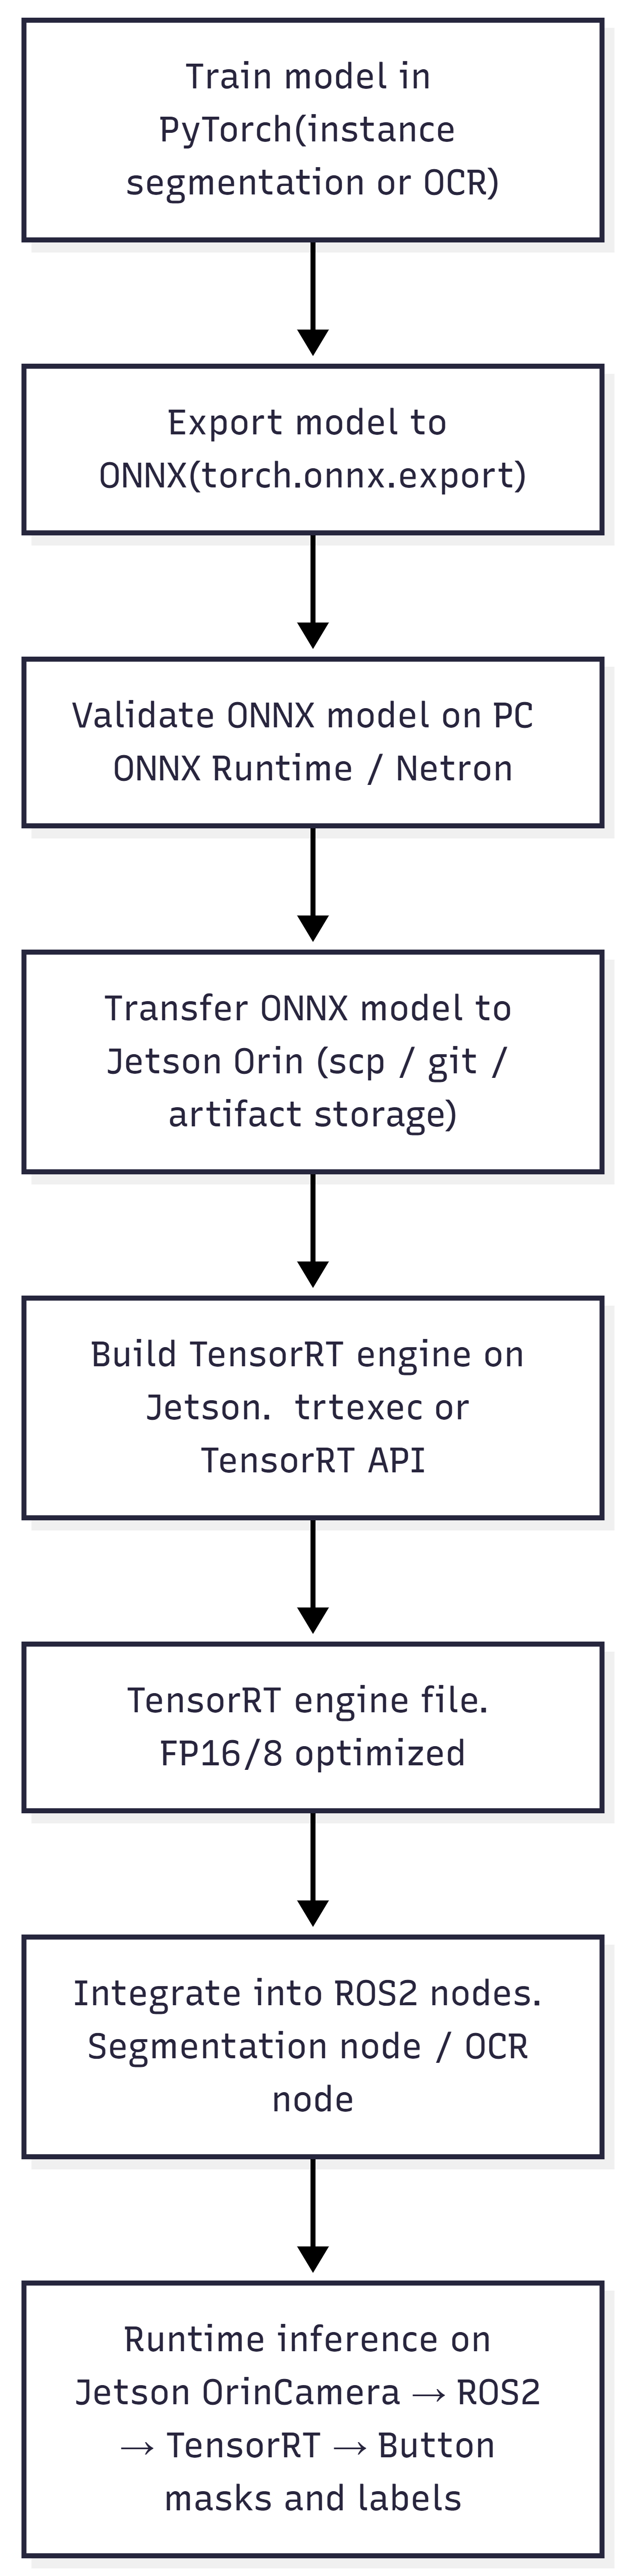
\includegraphics[width=0.25\textwidth]{figures/methodology/Embedded_workflow.png}
    \captionsetup{width=0.3\textwidth}
    \caption{Deployment and optimization workflow for 
    models on \gls{jetson} Orin using \gls{onnx} and \gls{tensorrt}.}
    \label{fig:tensorrt_workflow}
    \vspace{-10pt}
\end{wrapfigure}

To enable real-time execution on embedded hardware, and wrap up step 1 of the workflow strategy in Figure~\ref{fig:scalable_workflow}, trained models are optimized
and deployed on a \gls{jetson} Orin platform. The deployment workflow is designed
to be identical for both the instance segmentation model and the OCR-based button
classification model.

Models are first trained in PyTorch and exported to the Open Neural Network Exchange
(\gls{onnx}) \citep{onnx2019} format. The exported \gls{onnx} models are validated on a desktop system using \gls{onnx}
Runtime and model inspection tools to ensure numerical correctness and structural
compatibility prior to deployment.

Validated \gls{onnx} models are then transferred to the \gls{jetson} Orin device, where
\gls{tensorrt} is used to build optimized inference engines. Engine generation is
performed directly on the target device to ensure compatibility with the specific
\gls{gpu} architecture. \gls{fp16} precision is used to reduce memory footprint and improve
inference speed while maintaining sufficient numerical accuracy.

The resulting \gls{tensorrt} engines are integrated into \gls{ros2} nodes responsible for
perception tasks. At runtime, image data from the \gls{rgbd} camera is passed through
the \gls{ros2} pipeline and processed by the \gls{tensorrt} engines to produce instance
segmentation masks and corresponding button labels.

The complete deployment and optimization workflow is illustrated in
Figure~\ref{fig:tensorrt_workflow}. This approach ensures a consistent and efficient
deployment pipeline and enables fair evaluation of different model architectures
under identical runtime constraints.

